% !TEX program = pdflatex
\documentclass[aspectratio=169, 10pt]{beamer}

\usetheme{metropolis}

% ---------------------------------------------------------------------------
% COLOR & FONT TWEAKS
% ---------------------------------------------------------------------------
\definecolor{ColumbiaBlue}{HTML}{185494}
\definecolor{AccentOrange}{HTML}{E8792B}
\definecolor{LightGray}{HTML}{F5F5F5}
\definecolor{CodeBg}{HTML}{F0F0F0}
\definecolor{AlertRed}{HTML}{C0392B}
\definecolor{GoodGreen}{HTML}{27AE60}

\setbeamercolor{frametitle}{bg=ColumbiaBlue, fg=white}
\setbeamercolor{progress bar}{fg=AccentOrange}
\setbeamercolor{alerted text}{fg=AccentOrange}
\setbeamercolor{block title}{bg=ColumbiaBlue!15, fg=ColumbiaBlue}
\setbeamercolor{block body}{bg=ColumbiaBlue!5}
\setbeamercolor{block title alerted}{bg=AlertRed!15, fg=AlertRed}
\setbeamercolor{block body alerted}{bg=AlertRed!5}
\setbeamercolor{block title example}{bg=GoodGreen!15, fg=GoodGreen!80!black}
\setbeamercolor{block body example}{bg=GoodGreen!5}

\metroset{
  sectionpage=progressbar,
  subsectionpage=none,
  numbering=fraction,
  progressbar=frametitle,
  block=fill,
}

% ---------------------------------------------------------------------------
% PACKAGES
% ---------------------------------------------------------------------------
\usepackage{amsmath, amssymb, bm}
\usepackage{booktabs}
\usepackage{graphicx}
\usepackage{listings}
\usepackage{tikz}
\usetikzlibrary{arrows.meta, positioning, fit, calc, decorations.pathreplacing}
\usepackage{pifont}% for \ding checkmarks
\usepackage{xcolor}
\usepackage{hyperref}
\usepackage{appendixnumberbeamer}

% ---------------------------------------------------------------------------
% LISTINGS STYLE
% ---------------------------------------------------------------------------
\lstdefinestyle{python}{
  language=Python,
  basicstyle=\ttfamily\scriptsize,
  keywordstyle=\color{ColumbiaBlue}\bfseries,
  stringstyle=\color{AccentOrange},
  commentstyle=\color{gray}\itshape,
  backgroundcolor=\color{CodeBg},
  frame=single,
  framerule=0pt,
  xleftmargin=4pt,
  xrightmargin=4pt,
  aboveskip=6pt,
  belowskip=4pt,
  breaklines=true,
  showstringspaces=false,
}

% ---------------------------------------------------------------------------
% CUSTOM COMMANDS
% ---------------------------------------------------------------------------
% FIX: callout box as normal in-flow element (removed overlay/remember picture)
\newcommand{\notebookcallout}[2]{%
  \vspace{4pt}%
  \noindent\begin{tikzpicture}
    \node[
      fill=AccentOrange!10,
      draw=AccentOrange,
      rounded corners=4pt,
      inner sep=5pt,
      font=\scriptsize,
      text width=0.90\textwidth,
      align=left,
    ] {%
      {\color{AccentOrange}\ding{118}\;\textbf{Lab §#1}} — #2%
    };
  \end{tikzpicture}%
}

% Inline emphasis
\newcommand{\keyword}[1]{\textcolor{ColumbiaBlue}{\textbf{#1}}}
\newcommand{\bad}[1]{\textcolor{AlertRed}{#1}}
\newcommand{\good}[1]{\textcolor{GoodGreen!80!black}{#1}}

% Math shortcuts
\newcommand{\bbR}{\mathbb{R}}
\newcommand{\bx}{\bm{x}}
\newcommand{\bh}{\bm{h}}
\newcommand{\bW}{\bm{W}}
\newcommand{\bb}{\bm{b}}
\newcommand{\btheta}{\bm{\theta}}

% ---------------------------------------------------------------------------
% TITLE
% ---------------------------------------------------------------------------
\title{Neural Networks: From Motivation to Practice}
\subtitle{BINF 4002 --- Machine Learning for Health}
\author{Matthew McDermott}
\institute{Department of Biomedical Informatics, Columbia University}
\date{}

% ===================================================================
\begin{document}
% ===================================================================

\maketitle

% -------------------------------------------------------------------
\begin{frame}{Roadmap}

\begin{columns}[T]
\column{0.48\textwidth}
\begin{enumerate}
  \item \textbf{Motivation} --- why neural nets?
  \item \textbf{Anatomy} --- layers, activations, depth
  \item \textbf{Layer Types} --- architecture as bias
\end{enumerate}

\column{0.48\textwidth}
\begin{enumerate}\setcounter{enumi}{3}
  \item \textbf{Loss Functions} --- matching task to objective
  \item \textbf{Optimization} --- the practical toolkit
  \item \textbf{Putting It Together} --- recipe \& visualizations
\end{enumerate}
\end{columns}

\vspace{12pt}
\begin{center}
\small All experiments run live on MNIST in the companion notebook.\\
\textcolor{AccentOrange}{\ding{118}} \textbf{Notebook:} \texttt{nn\_fundamentals\_lab.ipynb}
\end{center}

\end{frame}

% ===================================================================
\section{Motivation}
% ===================================================================

% -------------------------------------------------------------------
\begin{frame}{What Do We Need From a Function Class?}

We want a \keyword{parametric function} $f_{\btheta}(\bx)$ that is simultaneously:

\begin{enumerate}
  \item<2-> \textbf{Arbitrarily expressive} --- can approximate any continuous mapping.
  \item<3-> \textbf{Parametric} --- fixed-size $\btheta$; doesn't grow with dataset.
  \item<4-> \textbf{Efficiently auto-differentiable} --- $\nabla_{\btheta}\mathcal{L}$ computable in $O(\text{forward pass})$.
\end{enumerate}

\vspace{6pt}

\onslide<5->{
\begin{alertblock}{Why all three?}
Health data is high-dimensional and nonlinear (expressiveness), models must be deployable (parametric), and we need scalable optimization (autodiff).
\end{alertblock}
}

\end{frame}

% -------------------------------------------------------------------
\begin{frame}{The Landscape of Alternatives}

\begin{table}
\centering
\small
\begin{tabular}{@{}lccc@{}}
\toprule
\textbf{Approach} & \textbf{Universal?} & \textbf{Parametric?} & \textbf{Autodiff?} \\
\midrule
Linear models        & \bad{\ding{55}} & \good{\ding{51}} & \good{\ding{51}} \\
\onslide<2->{Kernel / GP          & \good{\ding{51}} & \bad{\ding{55}} (grows w/ data) & \bad{\ding{55}} \\}
\onslide<3->{Trees / forests      & \good{\ding{51}} & $\sim$ (grows w/ depth) & \bad{\ding{55}} (discrete splits) \\}
\onslide<4->{\textbf{Neural nets} & \good{\ding{51}} & \good{\ding{51}} & \good{\ding{51}} \\}
\bottomrule
\end{tabular}
\end{table}

\vspace{8pt}
\onslide<4->{
\begin{exampleblock}{Key insight}
A neural network is a \textbf{composition of simple differentiable operations}. \\
The chain rule (autodiff) handles the rest.
\end{exampleblock}
}

\end{frame}

% ===================================================================
\section{Anatomy of a Neural Network}
% ===================================================================

% -------------------------------------------------------------------
\begin{frame}{The Fundamental Building Block: A Layer}

\begin{equation*}
  \boxed{\;\bh = \sigma\!\bigl(\bW\bx + \bb\bigr)\;}
\end{equation*}

\vspace{4pt}

\begin{columns}[T]
\column{0.48\textwidth}
\begin{itemize}
  \item $\bx \in \bbR^{d_{\text{in}}}$ --- input
  \item $\bW \in \bbR^{d_{\text{out}} \times d_{\text{in}}}$ --- weights
  \item $\bb \in \bbR^{d_{\text{out}}}$ --- bias
  \item $\sigma(\cdot)$ --- nonlinear activation
  \item $\bh \in \bbR^{d_{\text{out}}}$ --- output
\end{itemize}

\column{0.48\textwidth}
\textbf{Parameter count per layer:}
\[
  d_{\text{out}} \times d_{\text{in}} + d_{\text{out}}
\]

\vspace{6pt}
For $784 \to 256$: \quad $200{,}960$ parameters.
\end{columns}

\vspace{4pt}
\notebookcallout{1}{%
  \texttt{ManualMLP} class builds this with raw \texttt{nn.Parameter} tensors so you can see every matrix multiply.%
}

\end{frame}

% -------------------------------------------------------------------
\begin{frame}{Worked Example: Computing a Layer Output}

\small
\textbf{A tiny layer:} $d_{\text{in}}=3,\; d_{\text{out}}=2$, activation $= \text{ReLU}$.

\vspace{2pt}
\[
  \bW = \begin{pmatrix} 0.5 & -1.0 & 0.3 \\ 0.2 & 0.8 & -0.4 \end{pmatrix}, \quad
  \bb = \begin{pmatrix} 0.1 \\ -0.2 \end{pmatrix}, \quad
  \bx = \begin{pmatrix} 1 \\ 2 \\ 3 \end{pmatrix}
\]

\vspace{-6pt}
\onslide<2->{
\textbf{Step 1: Affine transform} $\bW\bx + \bb$

\vspace{-6pt}
\[
  \begin{pmatrix} 0.5(1) {+} (-1.0)(2) {+} 0.3(3) \\ 0.2(1) {+} 0.8(2) {+} (-0.4)(3) \end{pmatrix}
  + \begin{pmatrix} 0.1 \\ -0.2 \end{pmatrix}
  = \begin{pmatrix} -0.6 \\ 0.4 \end{pmatrix}
  + \begin{pmatrix} 0.1 \\ -0.2 \end{pmatrix}
  = \begin{pmatrix} \bad{-0.5} \\ \good{0.2} \end{pmatrix}
\]
}

\vspace{-8pt}
\onslide<3->{
\textbf{Step 2: ReLU} $\sigma(z) = \max(0, z)$
\qquad
$\bh = \bigl(\max(0,\;\bad{-0.5}),\;\;\max(0,\;\good{0.2})\bigr)^\top = (0,\;\;0.2)^\top$

\vspace{3pt}
Neuron 1 is \bad{dead} (ReLU kills the negative pre-activation). Neuron 2 passes through.
}

\end{frame}

% -------------------------------------------------------------------
\begin{frame}{Why the Nonlinearity is Essential}

Without $\sigma$, composing layers \textbf{collapses to a single linear map}:

\[
  \bh_2 = \bW_2(\bW_1 \bx + \bb_1) + \bb_2
        = \underbrace{(\bW_2\bW_1)}_{\tilde{\bW}}\bx
          + \underbrace{(\bW_2\bb_1 + \bb_2)}_{\tilde{\bb}}
\]

\vspace{4pt}

\onslide<2->{
\begin{table}
\centering\small
\begin{tabular}{@{}lll@{}}
\toprule
\textbf{Activation} & \textbf{Formula} & \textbf{Notes} \\
\midrule
ReLU    & $\max(0, x)$                    & Default. Simple, sparse, fast. \\
GELU    & $x\,\Phi(x)$                    & Smooth ReLU. Standard in transformers. \\
Sigmoid & $1/(1+e^{-x})$                  & Output $\in(0,1)$. Probability heads. \\
Tanh    & $(e^x-e^{-x})/(e^x+e^{-x})$    & Output $\in(-1,1)$. Centered sigmoid. \\
Softmax & $e^{x_i}/\!\sum_j e^{x_j}$     & Produces a distribution over classes. \\
\bottomrule
\end{tabular}
\end{table}
}

\end{frame}

% -------------------------------------------------------------------
\begin{frame}{Activations Impose Geometric Constraints}

The choice of activation determines what the layer \keyword{can and cannot represent}.

\vspace{4pt}
\begin{columns}[T]
\column{0.55\textwidth}
\textbf{ReLU zeroes the negative half-space.}

If all inputs are positive and all weights are positive, then $\bW\bx + \bb > 0$ and ReLU does nothing --- the layer is effectively linear.

\vspace{4pt}
\onslide<2->{
\textbf{Saturation kills gradients.}

Sigmoid/tanh saturate for large $|z|$: $\sigma'(z) \approx 0$. If many neurons saturate, gradients vanish.
}

\column{0.40\textwidth}
\begin{center}
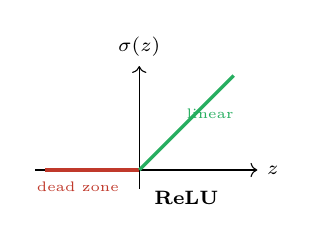
\begin{tikzpicture}[scale=0.6]
  % ReLU
  \draw[->] (-2.2,0) -- (2.5,0) node[right, font=\scriptsize]{$z$};
  \draw[->] (0,-0.4) -- (0,2.2) node[above, font=\scriptsize]{$\sigma(z)$};
  \draw[very thick, AlertRed] (-2,0) -- (0,0);
  \draw[very thick, GoodGreen] (0,0) -- (2,2);
  \node[font=\scriptsize\bfseries] at (1, -0.6) {ReLU};
  \node[font=\tiny, AlertRed] at (-1.3, -0.35) {dead zone};
  \node[font=\tiny, GoodGreen] at (1.5, 1.2) {linear};
\end{tikzpicture}
\end{center}

\vspace{-4pt}
\onslide<2->{
\begin{center}
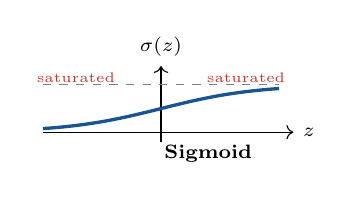
\begin{tikzpicture}[scale=0.6]
  \draw[->] (-2.5,0) -- (2.8,0) node[right, font=\scriptsize]{$z$};
  \draw[->] (0,-0.2) -- (0,1.4) node[above, font=\scriptsize]{$\sigma(z)$};
  \draw[very thick, ColumbiaBlue, domain=-2.5:2.5, samples=50] plot (\x, {1/(1+exp(-\x))});
  \draw[dashed, gray] (-2.5,1) -- (2.5,1);
  \node[font=\scriptsize\bfseries] at (1, -0.45) {Sigmoid};
  \node[font=\tiny, AlertRed] at (-1.8, 1.15) {saturated};
  \node[font=\tiny, AlertRed] at (1.8, 1.15) {saturated};
\end{tikzpicture}
\end{center}
}
\end{columns}

\onslide<3->{
\vspace{2pt}
\begin{exampleblock}{Rule of thumb}
\good{Default:} ReLU (or GELU for transformers). \;
\good{Final layer:} sigmoid for probabilities, softmax for multi-class, identity for regression.
\end{exampleblock}
}

\end{frame}

% -------------------------------------------------------------------
\begin{frame}{Composing Layers: A Deep Network}

\begin{align*}
  \bh_0 &= \bx \\
  \bh_\ell &= \sigma_\ell\!\bigl(\bW_\ell \bh_{\ell-1} + \bb_\ell\bigr)
    \qquad \ell = 1,\dots,L \\
  f_{\btheta}(\bx) &= \bh_L
\end{align*}

\vspace{4pt}

\begin{exampleblock}{Universal Approximation (Cybenko '89, Hornik '91)}
A single hidden layer of sufficient width can approximate any continuous function on a compact set.
\end{exampleblock}

\onslide<2->{
\vspace{2pt}
\textbf{But:} ``sufficient width'' may be \bad{exponentially large}. \\
\keyword{Depth} is far more parameter-efficient than width in practice. \\[4pt]
\emph{Intuition:} each layer learns a new coordinate system in which the remaining problem is simpler.
}

\end{frame}

% -------------------------------------------------------------------
\begin{frame}[fragile]{Reading Neural Network Diagrams}

\begin{columns}[T]

\column{0.30\textwidth}
\textbf{Style 1: Neuron-level}

\begin{center}
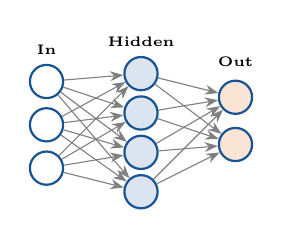
\begin{tikzpicture}[
  node distance=0.5cm and 1.0cm,
  neuron/.style={circle, draw=ColumbiaBlue, thick, minimum size=12pt, inner sep=0pt, font=\tiny},
  >=Stealth
]
  \foreach \i in {1,2,3}{
    \node[neuron] (i\i) at (0, -\i*0.55) {};
  }
  \foreach \j in {1,...,4}{
    \node[neuron, fill=ColumbiaBlue!15] (h\j) at (1.2, -\j*0.5+0.05) {};
  }
  \foreach \k in {1,2}{
    \node[neuron, fill=AccentOrange!20] (o\k) at (2.4, -\k*0.6-0.15) {};
  }
  \foreach \i in {1,2,3}
    \foreach \j in {1,...,4}
      \draw[->, thin, gray] (i\i) -- (h\j);
  \foreach \j in {1,...,4}
    \foreach \k in {1,2}
      \draw[->, thin, gray] (h\j) -- (o\k);

  \node[above=2pt, font=\tiny\bfseries] at (0, -0.4) {In};
  \node[above=2pt, font=\tiny\bfseries] at (1.2, -0.3) {Hidden};
  \node[above=2pt, font=\tiny\bfseries] at (2.4, -0.55) {Out};
\end{tikzpicture}
\end{center}
\scriptsize Circles = neurons, lines = weights.
Arrows show \emph{whether} info flows (nonzero $w$), not \emph{how much}. A missing arrow $=$ $w=0$ $=$ no information flow through that path.

\column{0.36\textwidth}
\textbf{Style 2: Block-level}

\begin{center}
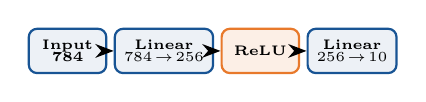
\begin{tikzpicture}[
  block/.style={rectangle, draw=ColumbiaBlue, thick, rounded corners=3pt,
    minimum height=16pt, minimum width=28pt, font=\fontsize{4.5}{5.5}\selectfont\bfseries,
    fill=ColumbiaBlue!8, align=center},
  >=Stealth, node distance=0.08cm
]
  \node[block] (in) {Input\\[-1pt]784};
  \node[block, right=of in] (l1) {Linear\\[-1pt]$784\!\to\!256$};
  \node[block, right=of l1, fill=AccentOrange!12, draw=AccentOrange] (r1) {ReLU};
  \node[block, right=of r1] (l2) {Linear\\[-1pt]$256\!\to\!10$};
  \draw[->, thick] (in) -- (l1);
  \draw[->, thick] (l1) -- (r1);
  \draw[->, thick] (r1) -- (l2);
\end{tikzpicture}
\end{center}
\scriptsize Blocks = operations.\\
This is what papers typically use.

\column{0.30\textwidth}
\textbf{Style 3: Code-level}

\begin{lstlisting}[style=python, basicstyle=\ttfamily\fontsize{5.5}{7}\selectfont]
nn.Sequential(
  nn.Linear(784, 256),
  nn.ReLU(),
  nn.Linear(256, 10),
)
\end{lstlisting}

\vspace{4pt}
\scriptsize The diagram \emph{is} the code. \\
PyTorch reads like an architecture spec.

\end{columns}

\end{frame}

% ===================================================================
\section{Layer Types as Inductive Biases}
% ===================================================================

% -------------------------------------------------------------------
\begin{frame}{Architecture Encodes Assumptions}

\begin{table}
\centering\small
\begin{tabular}{@{}p{2.2cm}p{4.5cm}p{5.5cm}@{}}
\toprule
\textbf{Layer Type} & \textbf{Core Assumption} & \textbf{Operation} \\
\midrule
Fully connected & No structural assumption & $\bh = \sigma(\bW\bx + \bb)$ \\[4pt]
Convolutional & Local, translation-equivariant & $h_i = \sigma\!\bigl(\sum_k w_k \cdot x_{i+k} + b\bigr)$ \\[4pt]
Recurrent (RNN) & Sequential; hidden state summary & $\bh_t = \sigma(\bW_h \bh_{t-1} + \bW_x \bx_t + \bb)$ \\[4pt]
Attention & Set-like; learned interactions & $\text{softmax}\!\bigl(\frac{QK^\top}{\sqrt{d_k}}\bigr)V$ \\
\bottomrule
\end{tabular}
\end{table}

\vspace{6pt}
The choice of layer type determines what the model \keyword{can easily learn} vs.\ what it must \bad{fight to learn}.

\end{frame}

% -------------------------------------------------------------------
\begin{frame}{How Layer Types Differ: Connectivity Patterns}

\begin{columns}[T]

\column{0.30\textwidth}
\textbf{Fully Connected}

\begin{center}
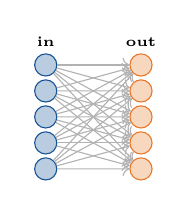
\begin{tikzpicture}[scale=0.55,
  in_node/.style={circle, fill=ColumbiaBlue!30, draw=ColumbiaBlue, minimum size=8pt, inner sep=0pt},
  out_node/.style={circle, fill=AccentOrange!30, draw=AccentOrange, minimum size=8pt, inner sep=0pt},
]
  \foreach \i in {1,...,5} { \node[in_node] (i\i) at (0, -\i*0.6) {}; }
  \foreach \j in {1,...,5} { \node[out_node] (o\j) at (2.2, -\j*0.6) {}; }
  \foreach \i in {1,...,5}
    \foreach \j in {1,...,5}
      \draw[->, thin, gray!60] (i\i) -- (o\j);
  \node[font=\tiny\bfseries, above] at (0, -0.4) {in};
  \node[font=\tiny\bfseries, above] at (2.2, -0.4) {out};
\end{tikzpicture}
\end{center}
\scriptsize Every input connects to every output. No structural prior.

\column{0.30\textwidth}
\textbf{Convolutional}

\begin{center}
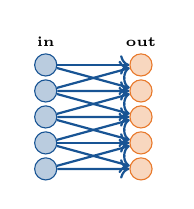
\begin{tikzpicture}[scale=0.55,
  in_node/.style={circle, fill=ColumbiaBlue!30, draw=ColumbiaBlue, minimum size=8pt, inner sep=0pt},
  out_node/.style={circle, fill=AccentOrange!30, draw=AccentOrange, minimum size=8pt, inner sep=0pt},
]
  \foreach \i in {1,...,5} { \node[in_node] (i\i) at (0, -\i*0.6) {}; }
  \foreach \j in {1,...,5} { \node[out_node] (o\j) at (2.2, -\j*0.6) {}; }
  % local connections only (kernel size 3)
  \foreach \j in {1,...,5}{
    \pgfmathtruncatemacro{\lo}{max(1, \j-1)}
    \pgfmathtruncatemacro{\hi}{min(5, \j+1)}
    \foreach \i in {\lo,...,\hi}
      \draw[->, thick, ColumbiaBlue] (i\i) -- (o\j);
  }
  \node[font=\tiny\bfseries, above] at (0, -0.4) {in};
  \node[font=\tiny\bfseries, above] at (2.2, -0.4) {out};
\end{tikzpicture}
\end{center}
\scriptsize Each output sees only a \keyword{local window}. Same weights reused at every position.

\column{0.36\textwidth}
\textbf{Attention}

\begin{center}
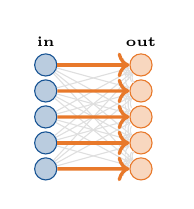
\begin{tikzpicture}[scale=0.55,
  tok/.style={circle, fill=ColumbiaBlue!30, draw=ColumbiaBlue, minimum size=8pt, inner sep=0pt},
  out_tok/.style={circle, fill=AccentOrange!30, draw=AccentOrange, minimum size=8pt, inner sep=0pt},
]
  \foreach \i in {1,...,5} { \node[tok] (i\i) at (0, -\i*0.6) {}; }
  \foreach \j in {1,...,5} { \node[out_tok] (o\j) at (2.2, -\j*0.6) {}; }
  % all-to-all (faint) — fully connected like FC
  \foreach \i in {1,...,5}
    \foreach \j in {1,...,5}
      \draw[->, thin, gray!25] (i\i) -- (o\j);
  % highlight diagonal (self-connection): token attends most to itself
  \foreach \i in {1,...,5}
    \draw[->, very thick, AccentOrange] (i\i) -- (o\i);
  \node[font=\tiny\bfseries, above] at (0, -0.4) {in};
  \node[font=\tiny\bfseries, above] at (2.2, -0.4) {out};
\end{tikzpicture}
\end{center}
\scriptsize Structurally fully connected, but weights are \keyword{learned \& input-dependent}. Highlighted: each token's strongest self-attention.

\end{columns}

\end{frame}

% -------------------------------------------------------------------
\begin{frame}{Mapping Architecture to Clinical Domain}

\begin{table}
\centering\small
\begin{tabular}{@{}lll@{}}
\toprule
\textbf{Data Modality} & \textbf{Typical Architecture} & \textbf{Why} \\
\midrule
Tabular / EHR features  & MLP or Transformer     & No spatial/sequential structure \\
Medical images           & CNN (ResNet, etc.)      & Spatial locality, translation invariance \\
Clinical notes           & Transformer             & Long-range dependencies \\
Vitals / waveforms       & CNN or Transformer      & Local temporal patterns \\
EHR event sequences      & Transformer             & Variable-length, irregular timing \\
Molecular graphs         & GNN                     & Relational structure \\
\bottomrule
\end{tabular}
\end{table}

\onslide<2->{
\vspace{4pt}
\begin{exampleblock}{Rule of thumb}
\good{Not sure?} Start with a Transformer --- fewest structural assumptions. \\
\good{Small data?} MLP or logistic regression may outperform deep models.
\end{exampleblock}
}

\end{frame}

% ===================================================================
\section{Loss Functions}
% ===================================================================

% -------------------------------------------------------------------
\begin{frame}{Choosing a Loss Function}

The loss $\mathcal{L}\bigl(f_{\btheta}(\bx),\, y\bigr)$ measures how wrong the model is. The choice depends on the \keyword{task}:

\vspace{6pt}
\begin{table}
\centering\small
\begin{tabular}{@{}p{2.6cm}p{5.8cm}l@{}}
\toprule
\textbf{Task} & \textbf{Loss} & \textbf{Final act.} \\
\midrule
Binary classif. & Binary CE: $-\bigl[y\log\hat{y}+(1\!-\!y)\log(1\!-\!\hat{y})\bigr]$ & Sigmoid \\[6pt]
Multi-class & Cross-entropy: $-\sum_c y_c \log \hat{y}_c$ & Softmax \\[6pt]
Regression & MSE: $(y - \hat{y})^2$ & Identity \\[6pt]
Survival & Negative partial log-likelihood & Varies \\
\bottomrule
\end{tabular}
\end{table}

\vspace{2pt}
\onslide<2->{
\begin{exampleblock}{Unifying view: every loss above is a negative log-likelihood}
Binary CE $=$ NLL of a Bernoulli. \\
Cross-entropy $=$ NLL of a Categorical. \\
MSE $=$ NLL of a Gaussian (up to a constant). \\
Survival loss is already a partial NLL. \\[2pt]
Choosing a loss $\Leftrightarrow$ choosing a probabilistic model for $p(y \mid \bx)$.
\end{exampleblock}
}

\end{frame}

% ===================================================================
\section{Optimization in Practice}
% ===================================================================

% -------------------------------------------------------------------
\begin{frame}{This Is Where Projects Succeed or Fail}

Theory gives us SGD.
Practice requires a \keyword{constellation of techniques}:

\vspace{4pt}
\begin{columns}[T]
\column{0.48\textwidth}
\begin{enumerate}
  \item Initialization
  \item Normalization
  \item Residual connections
  \item Optimizer choice
  \item Learning rate \& schedules
\end{enumerate}

\column{0.48\textwidth}
\begin{enumerate}\setcounter{enumi}{5}
  \item LR $\leftrightarrow$ batch size relationship
  \item Gradient clipping
  \item Gradient accumulation
  \item Monitoring (wandb)
  \item Regularization
\end{enumerate}
\end{columns}

\vspace{8pt}
Each of the following slides covers one topic. \\
The \textcolor{AccentOrange}{\ding{118}} \textbf{lab callouts} point you to live experiments.

\end{frame}

% -------------------------------------------------------------------
\subsection{Initialization}
% -------------------------------------------------------------------
\begin{frame}{1.\ \ Why Does Initialization Matter?}

\textbf{Goal:} at init, every layer should produce outputs with \keyword{roughly the same variance} as its inputs.

\vspace{8pt}
\onslide<2->{
\textbf{But why?} Consider a deep network with $L$ layers. If each layer scales its input variance by a factor $\alpha$:
\[
  \text{Var}(\bh_L) \;=\; \alpha^L \;\text{Var}(\bx)
\]
}

\onslide<3->{
\vspace{4pt}
\begin{alertblock}{The exponential amplification problem}
\bad{$\alpha > 1$}: variance explodes exponentially with depth $\to$ NaN activations/gradients. \\
\bad{$\alpha < 1$}: variance collapses exponentially $\to$ all activations $\approx 0$, no learning. \\[2pt]
\good{$\alpha = 1$}: variance preserved across layers --- \textbf{this is the target.}
\end{alertblock}
}

\onslide<4->{
\vspace{4pt}
The right initialization \emph{sets} $\alpha \approx 1$ by choosing weight variance as a function of layer width.
}

\end{frame}

% -------------------------------------------------------------------
\begin{frame}{1.\ \ Initialization --- Strategies}

\begin{columns}[T]
\column{0.52\textwidth}
\textbf{Xavier / Glorot} (tanh, sigmoid):
\[
  W_{ij} \sim \mathcal{N}\!\Bigl(0,\;\frac{2}{d_{\text{in}}+d_{\text{out}}}\Bigr)
\]

\textbf{Kaiming / He} (ReLU):
\[
  W_{ij} \sim \mathcal{N}\!\Bigl(0,\;\frac{2}{d_{\text{in}}}\Bigr)
\]

\column{0.44\textwidth}
\onslide<2->{
\begin{alertblock}{What goes wrong}
\bad{Too large} $\to$ activations/gradients explode \\
\bad{Too small} $\to$ activations collapse to 0 \\
\bad{All zeros} $\to$ symmetry never broken
\end{alertblock}
}
\end{columns}

\onslide<3->{
\vspace{4pt}
\textbf{Why these formulas?} If $\text{Var}(x_j) = v$ and weights are i.i.d.\ with variance $\sigma^2$, then $\text{Var}(\sum_j W_{ij}x_j) = d_\text{in}\,\sigma^2\,v$. Setting $\sigma^2 = 1/d_\text{in}$ (Xavier) or $2/d_\text{in}$ (Kaiming, accounting for ReLU halving) keeps output variance $\approx$ input variance.
}

\end{frame}

% -------------------------------------------------------------------
\begin{frame}{1.\ \ Initialization --- Lab Results}

\begin{center}
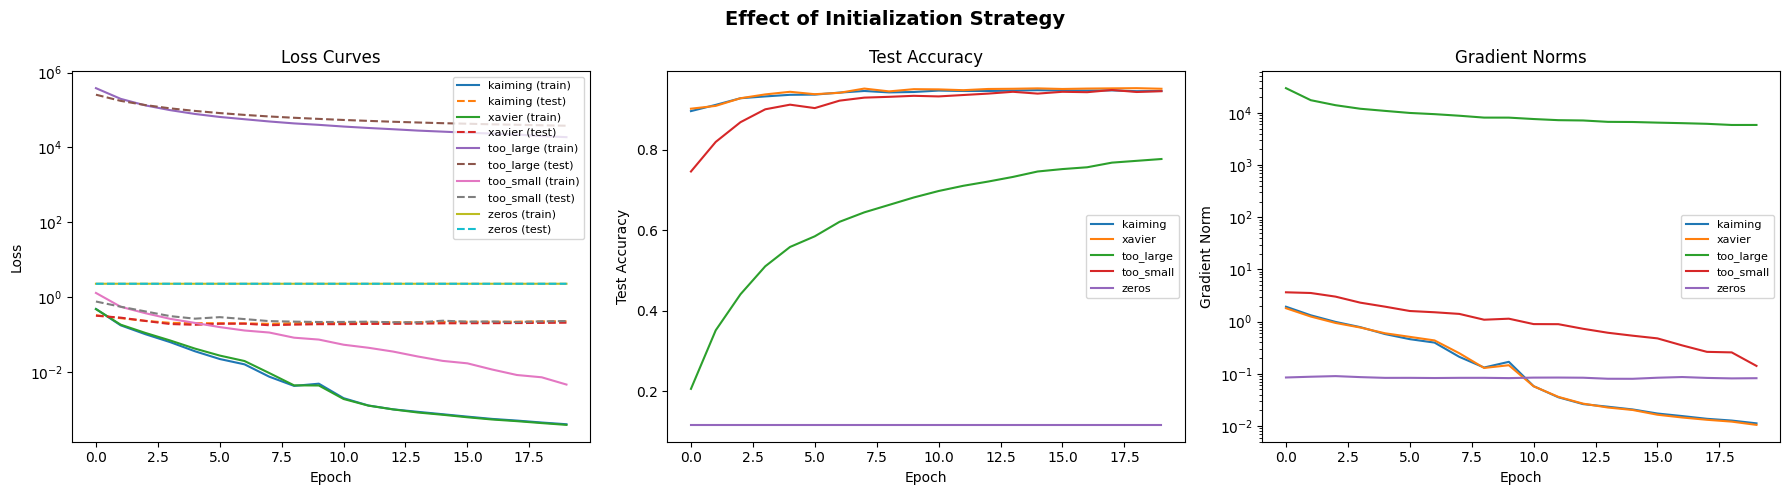
\includegraphics[width=\textwidth]{figures/initialization_experiment.png}
\end{center}

\vspace{2pt}
\small
\good{Kaiming} and \good{Xavier} converge to $>95\%$ accuracy.
\bad{Too-large} init ($\sigma\!=\!5$) causes exploding gradients ($>10^3$, right panel).
\bad{Too-small} ($\sigma\!=\!10^{-4}$) and \bad{zeros} never escape their starting point --- loss flatlines.

\notebookcallout{4}{%
  Five strategies on the same 3-layer MLP / MNIST. \textbf{Try it:} swap \texttt{kaiming} $\to$ \texttt{zeros} and watch accuracy flatline.%
}

\end{frame}

% -------------------------------------------------------------------
\subsection{Normalization}
% -------------------------------------------------------------------
\begin{frame}{2.\ \ Normalization --- The Problem}

Even with good init, activation distributions \textbf{drift} during training --- this is called \keyword{internal covariate shift}.

\vspace{2pt}
\begin{center}
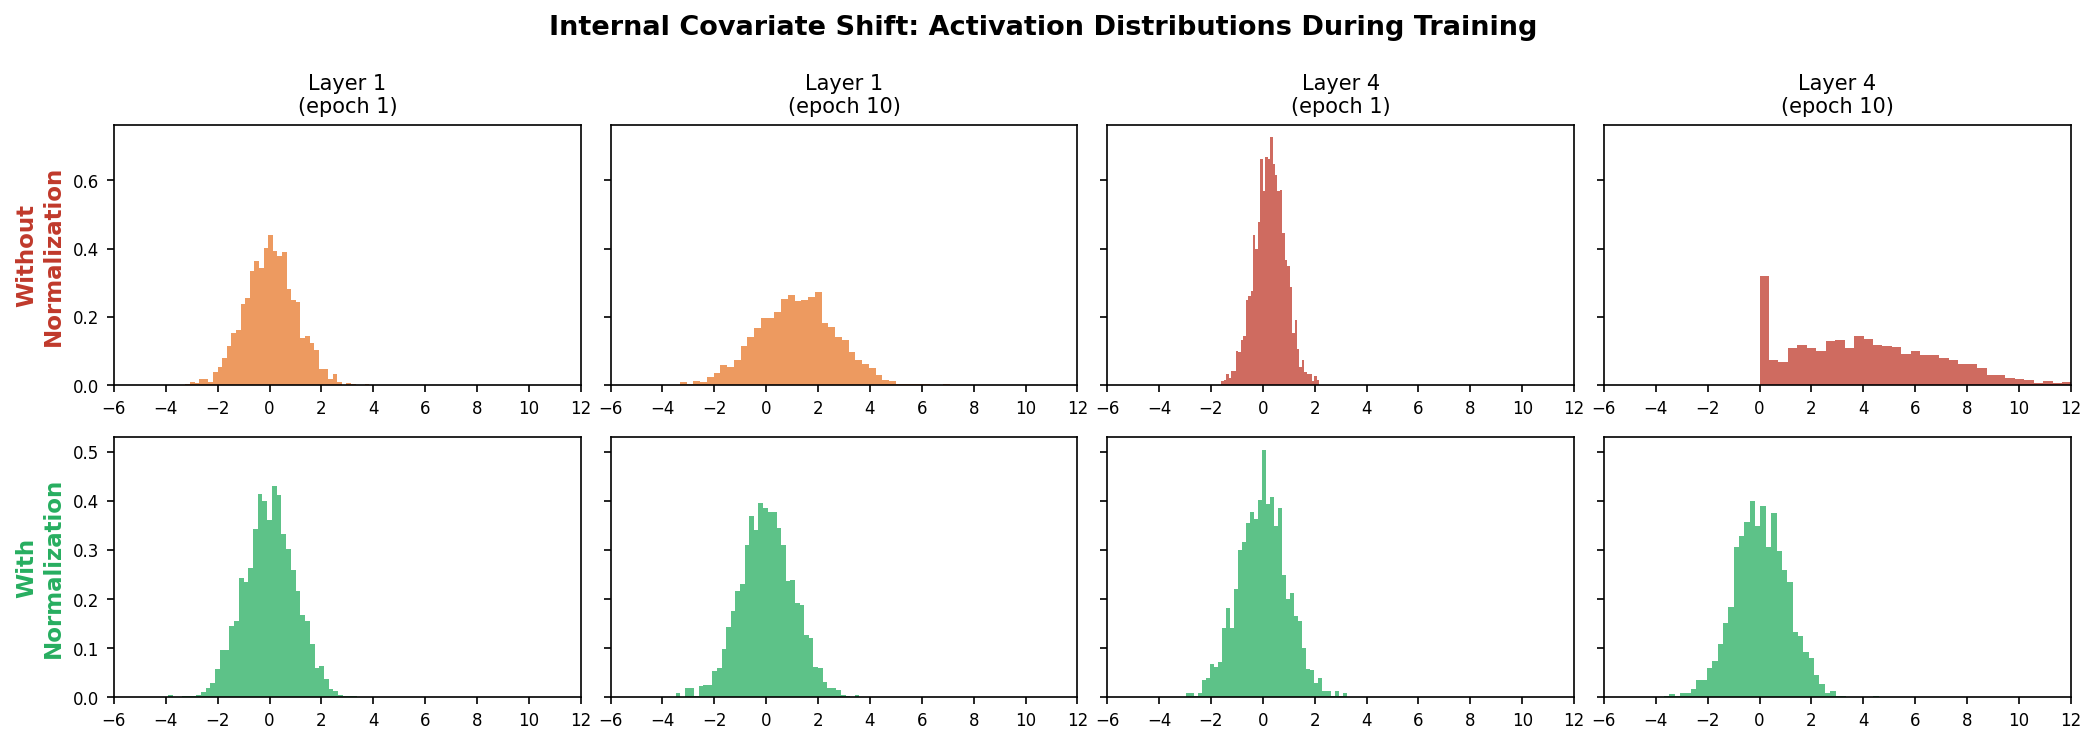
\includegraphics[width=0.85\textwidth]{figures/activation_drift.png}
\end{center}

\vspace{2pt}
\small
Without normalization, later layers must constantly re-adapt to shifting input distributions.
Normalization forces each layer's inputs to have stable statistics.

\end{frame}

% -------------------------------------------------------------------
\begin{frame}{2.\ \ Normalization --- Methods}

\begin{columns}[T]
\column{0.48\textwidth}
\textbf{Batch Normalization}
\[
  \hat{x}_i = \frac{x_i - \mu_B}{\sqrt{\sigma_B^2 + \epsilon}},
  \qquad y_i = \gamma\hat{x}_i + \beta
\]
Normalize across the \emph{batch} per feature. \\
$\gamma, \beta$ are learned. \\[4pt]
\scriptsize Caveat: train/test behavior differs (running stats).

\column{0.48\textwidth}
\textbf{Layer Normalization}
\[
  \hat{x}_i = \frac{x_i - \mu_\text{layer}}{\sqrt{\sigma_\text{layer}^2 + \epsilon}}
\]
Normalize across \emph{features} per example. \\
No batch dependence. \\[4pt]
\scriptsize Standard in transformers.
\end{columns}

\onslide<2->{
\vspace{4pt}
\begin{exampleblock}{Rule of thumb}
\good{CNNs?} BatchNorm (after conv, before activation). \\
\good{Transformers?} LayerNorm. \\
\good{Small/variable batches?} LayerNorm or GroupNorm.
\end{exampleblock}
}

\onslide<3->{
\vspace{2pt}
\scriptsize \textbf{Historical note:} Self-Normalizing Networks (Klambauer et al., 2017) used the SELU activation to maintain stable distributions without explicit normalization layers. Elegant in theory, but rarely used today --- explicit normalization is simpler and more robust.
}

\end{frame}

% -------------------------------------------------------------------
\subsection{Residual Connections}
% -------------------------------------------------------------------
\begin{frame}{3.\ \ Residual Connections}

\textbf{The degradation problem:} naively, deeper $\neq$ better. A 20-layer plain net can train \bad{worse} than a 5-layer net.

\vspace{4pt}

\begin{columns}[T]
\column{0.55\textwidth}
\textbf{The fix (He et al., 2015):}
\[
  \bh_{\ell+1} = \bh_\ell + F(\bh_\ell)
\]

\begin{itemize}
  \item Identity is the \keyword{default} (set $F=0$).
  \item Gradients flow directly through skip: $\frac{\partial \bh_L}{\partial \bh_\ell} = I + \cdots$
  \item Enabled 100+ layer training (ResNet).
\end{itemize}

\column{0.40\textwidth}
\begin{center}
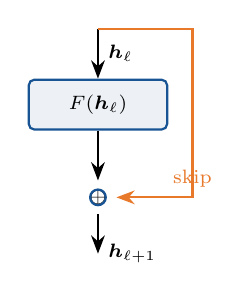
\begin{tikzpicture}[
  block/.style={rectangle, draw=ColumbiaBlue, thick, rounded corners=2pt,
    minimum height=18pt, minimum width=50pt, font=\scriptsize\bfseries,
    fill=ColumbiaBlue!8},
  >=Stealth
]
  \node[block] (f) {$F(\bh_\ell)$};
  \node[below=18pt of f, font=\scriptsize] (plus) {$\oplus$};
  \node[circle, draw=ColumbiaBlue, thick, inner sep=2pt] at (plus) {};

  \draw[->, thick] ([yshift=18pt]f.north) -- (f.north) node[midway, right, font=\scriptsize]{$\bh_\ell$};
  \draw[->, thick] (f.south) -- (plus.north);
  \draw[->, thick, AccentOrange] ([yshift=18pt]f.north) -- ++(1.2,0) |- (plus.east) node[midway, above, font=\scriptsize, text=AccentOrange]{skip};
  \draw[->, thick] (plus.south) -- ++(0,-0.5) node[right, font=\scriptsize]{$\bh_{\ell+1}$};
\end{tikzpicture}
\end{center}
\end{columns}

\notebookcallout{5}{%
  Depth experiment compares 3-layer baseline, 10-layer plain, + BN, + LN, + residual, + BN + residual.%
}

\end{frame}

% -------------------------------------------------------------------
\begin{frame}{3.\ \ Residual Connections --- Deeper Interpretations}

Beyond ``gradient highway,'' residual connections have richer interpretations:

\vspace{6pt}
\begin{itemize}
  \item<2-> \textbf{Ensemble of paths} (Veit et al., 2016): A ResNet of $L$ blocks has $2^L$ paths from input to output. Empirically, most gradient signal flows through \emph{short} paths --- the network behaves like an ensemble of shallow networks.

  \item<3-> \textbf{Iterative refinement:} Each block computes a small \emph{correction} $F(\bh_\ell)$ to the current representation, rather than building a new one from scratch.

  \item<4-> \textbf{Unrolled optimization:} Deep equilibrium models (Bai et al., 2019) show residual blocks can be viewed as steps of an implicit fixed-point iteration: $\bh^* = \bh^* + F(\bh^*)$.
\end{itemize}

\onslide<5->{
\vspace{6pt}
\scriptsize \textbf{References:}
Veit et al., ``Residual Networks Behave Like Ensembles of Relatively Shallow Networks'' (NeurIPS 2016); \;
Bai et al., ``Deep Equilibrium Models'' (NeurIPS 2019).
}

\end{frame}

% -------------------------------------------------------------------
\begin{frame}{3.\ \ Depth, Normalization \& Residuals --- Lab Results}

\begin{center}
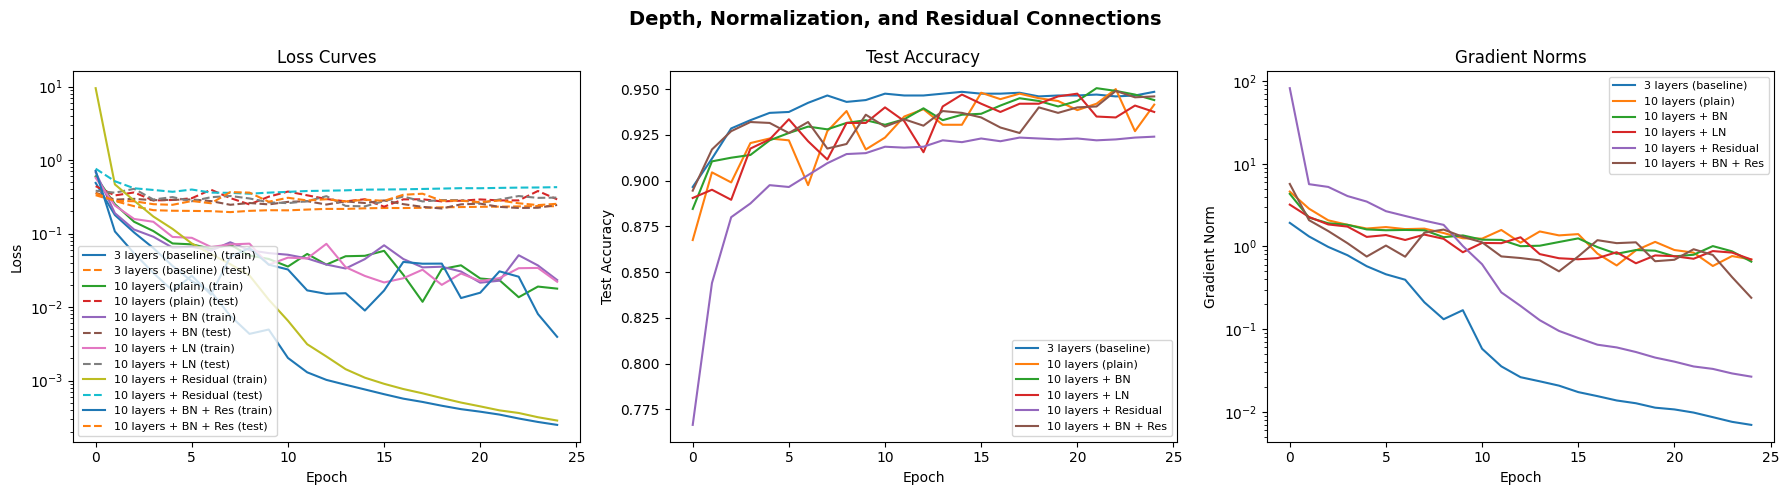
\includegraphics[width=\textwidth]{figures/depth_experiment.png}
\end{center}

\vspace{2pt}
\small
The plain 10-layer net \bad{degrades} below the shallow 3-layer baseline (the ``degradation problem'').
Adding \good{BatchNorm + residuals} recovers and surpasses it --- reaching the highest accuracy.
Right panel: normalization keeps gradient norms stable across depth.

\end{frame}

% -------------------------------------------------------------------
\subsection{Optimizers}
% -------------------------------------------------------------------
\begin{frame}{4.\ \ Optimizers: Beyond Vanilla SGD}

\begin{columns}[T]
\column{0.48\textwidth}
\textbf{SGD + Momentum}
\begin{align*}
  v_t &= \beta\, v_{t-1} + \nabla_{\btheta}\mathcal{L} \\
  \btheta_t &= \btheta_{t-1} - \eta\, v_t
\end{align*}
Smooths noisy gradients; accelerates along consistent directions.

\column{0.48\textwidth}
\textbf{Adam / AdamW}
\begin{align*}
  m_t &= \beta_1 m_{t-1} + (1-\beta_1)\,g_t \\
  v_t &= \beta_2 v_{t-1} + (1-\beta_2)\,g_t^2 \\
  \btheta_t &= \btheta_{t-1} - \eta\,\frac{\hat m_t}{\sqrt{\hat v_t}+\epsilon}
\end{align*}
Per-parameter adaptive LR.  Robust default.
\end{columns}

\vspace{8pt}
\onslide<2->{
\begin{exampleblock}{Rule of thumb}
\good{Starting out?} AdamW, $\eta=10^{-3}$. \\
\good{Transformers?} AdamW. \\
\good{Vision SOTA?} SGD + momentum can edge ahead with careful tuning.
\end{exampleblock}
}

\end{frame}

% -------------------------------------------------------------------
\subsection{Learning Rate}
% -------------------------------------------------------------------
\begin{frame}{5.\ \ Learning Rate: The Most Important Hyperparameter}

\begin{columns}[T]
\column{0.35\textwidth}
\bad{Too high} $\to$ divergence \\[2pt]
\good{Just right} $\to$ smooth convergence \\[2pt]
\bad{Too low} $\to$ painfully slow

\vspace{8pt}
\textbf{First thing to sweep:}
\[
  \eta \in \{10^{-4},\, 3\!\times\!10^{-4},\, 10^{-3},\, 3\!\times\!10^{-3}\}
\]

\column{0.60\textwidth}
\textbf{Common schedules:}

\vspace{2pt}
{\small\begin{tabular}{@{}lp{5.2cm}@{}}
\toprule
Step decay & Drop by $\gamma$ every $N$ epochs \\[2pt]
Cosine & $\eta_t \!=\! \eta_{\min} + \tfrac{1}{2}(\eta_{\max}\!-\!\eta_{\min})(1\!+\!\cos\tfrac{\pi t}{T})$ \\[2pt]
Warmup + decay & Ramp up, then cosine/linear down \\
\bottomrule
\end{tabular}}

\vspace{6pt}
\textbf{Why warmup?} Early gradients are high-variance (random weights). Low initial LR prevents destructive updates.
\end{columns}

\vspace{4pt}
\onslide<2->{
\begin{alertblock}{Why decay is necessary}
Convergence theory (Robbins--Monro) requires $\sum \eta_t = \infty$ (reach the optimum) and $\sum \eta_t^2 < \infty$ (don't oscillate past it). A constant LR violates the second condition --- you \emph{must} decay.
\end{alertblock}
}

\end{frame}

% -------------------------------------------------------------------
\begin{frame}{5.\ \ Learning Rate --- Lab Results}

\begin{center}
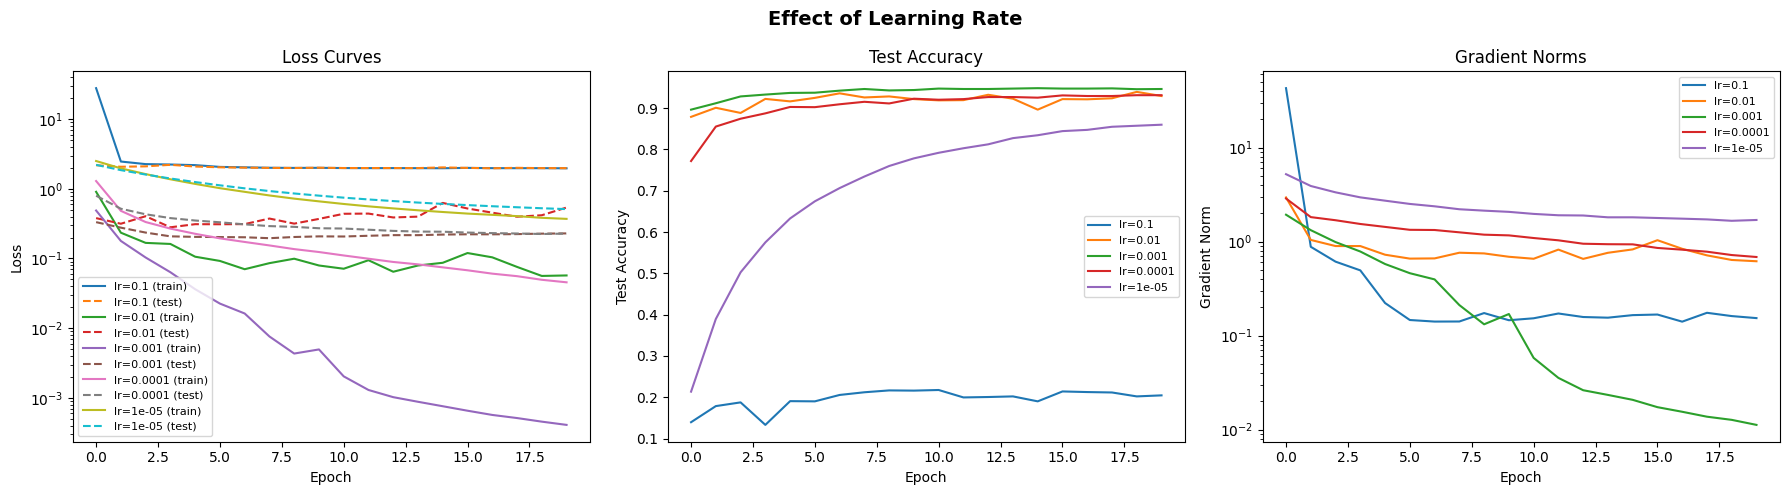
\includegraphics[width=\textwidth]{figures/lr_sweep.png}
\end{center}

\vspace{2pt}
\small
$\eta=10^{-1}$: \bad{diverges} (loss spikes, accuracy crashes).
$\eta=10^{-5}$: \bad{too slow} (barely learns in 20 epochs).
$\eta\in\{10^{-2}, 10^{-3}\}$: \good{sweet spot} --- fast convergence, high accuracy.

\notebookcallout{6}{%
  LR sweep: trains with $\eta\in\{10^{-1}, 10^{-2}, 10^{-3}, 10^{-4}, 10^{-5}\}$.%
}

\end{frame}

% -------------------------------------------------------------------
\begin{frame}{5.\ \ Learning Rate Schedules --- Lab Results}

\begin{center}
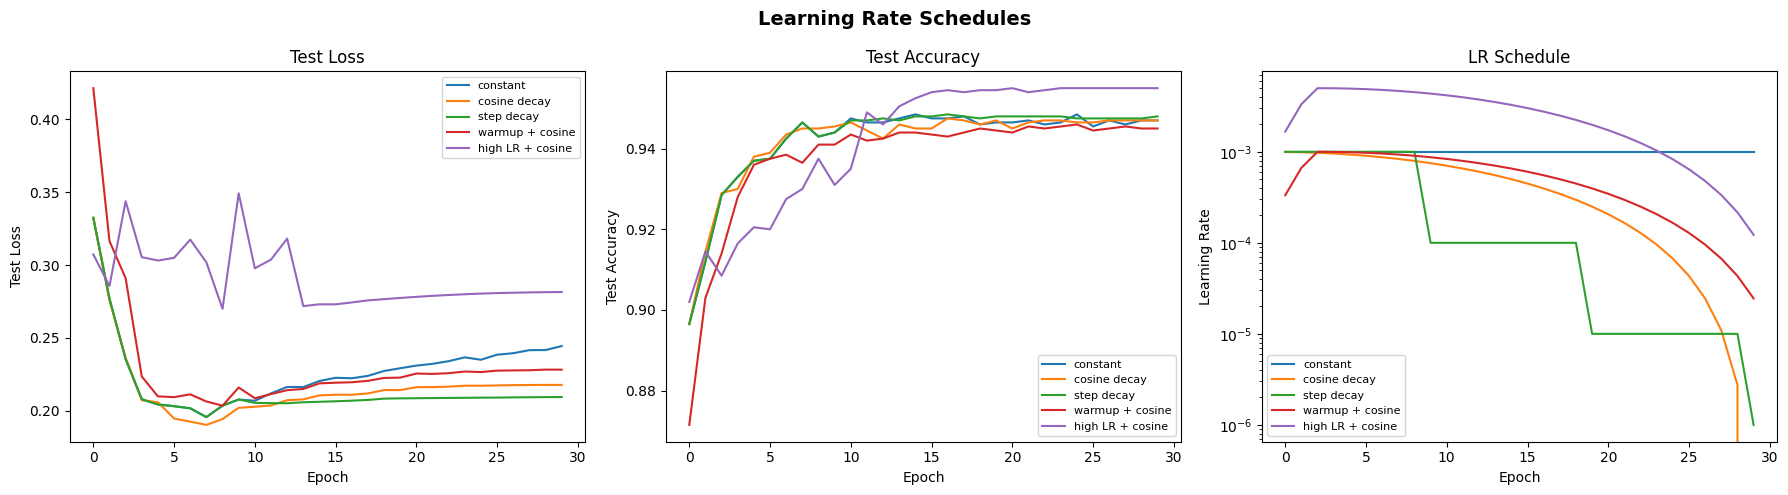
\includegraphics[width=\textwidth]{figures/lr_schedules.png}
\end{center}

\vspace{2pt}
\small
Cosine and step decay outperform constant LR on test loss.
Warmup + cosine is most stable early on.
Right panel: the actual LR trajectory for each schedule.

\notebookcallout{7}{%
  Schedule comparison: constant vs.\ cosine vs.\ step vs.\ warmup + cosine.%
}

\end{frame}

% -------------------------------------------------------------------
\subsection{Batch Size \& LR Scaling}
% -------------------------------------------------------------------
\begin{frame}{6.\ \ The Learning Rate --- Batch Size Relationship}

\begin{block}{Linear Scaling Rule (Goyal et al., 2017)}
When you multiply batch size by $k$, multiply learning rate by $k$:
\[
  \eta_{\text{new}} = \eta_{\text{base}} \times \frac{B_{\text{new}}}{B_{\text{base}}}
\]
\end{block}

\textbf{Intuition:} larger batch $\to$ lower-variance gradient $\to$ can take bigger steps.

\vspace{4pt}
\onslide<2->{
\begin{alertblock}{Practical implication}
If you change GPU and therefore batch size, \textbf{always} rescale LR. \\
Gradient accumulation changes effective batch size too.
\end{alertblock}
}

\notebookcallout{8}{%
  Batch size experiment: compares baseline, wrong (same LR), correctly scaled, and scaled down.%
}

\end{frame}

% -------------------------------------------------------------------
\begin{frame}{6.\ \ Batch Size \& LR Scaling --- Lab Results}

\begin{center}
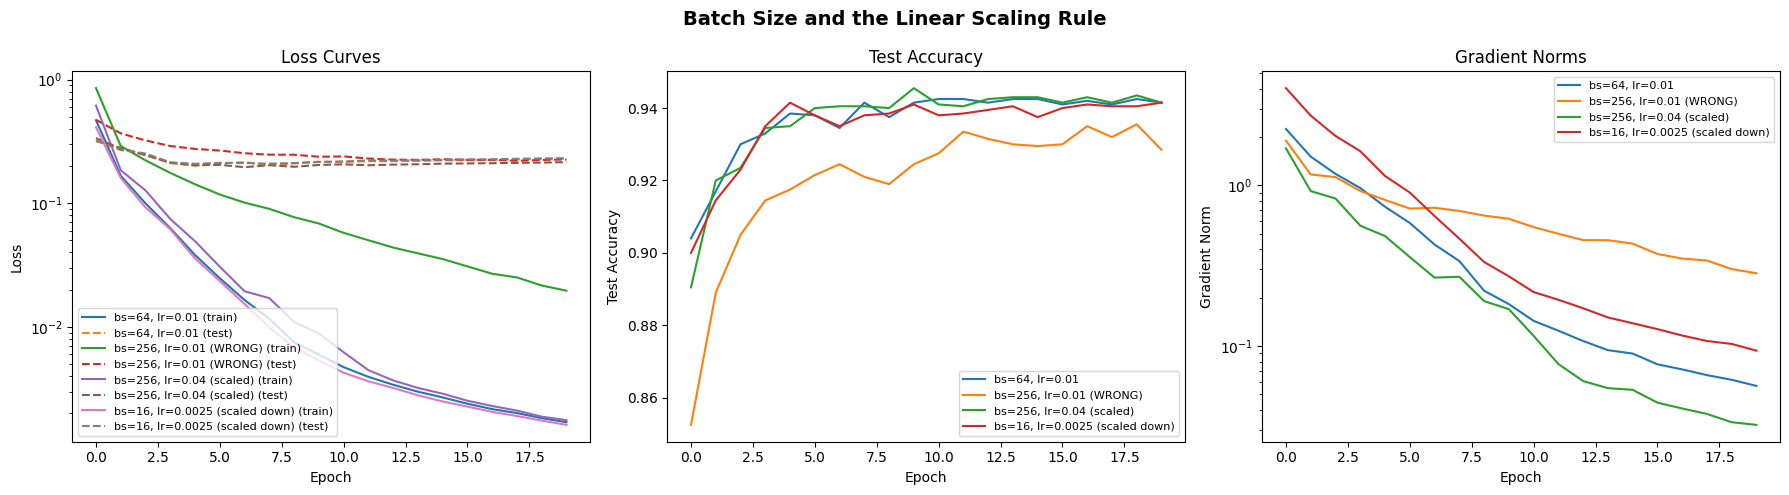
\includegraphics[width=\textwidth]{figures/batch_size_experiment.png}
\end{center}

\vspace{2pt}
\small
\bad{bs=256, lr=0.001 (WRONG)}: fewer steps per epoch \emph{and} same step size $\to$ under-trains.
\good{bs=256, lr=0.004 (scaled)}: $4\times$ larger LR compensates for $4\times$ fewer steps --- matches the baseline.
The scaled-down run (bs=16) also tracks correctly.

\end{frame}

% -------------------------------------------------------------------
\subsection{Gradient Clipping}
% -------------------------------------------------------------------
\begin{frame}{7.\ \ Gradient Clipping}

\textbf{Problem:} gradient norms can \bad{spike} $\to$ destructive parameter updates.

\vspace{4pt}
\textbf{Fix --- norm clipping:}
\[
  \nabla_{\btheta}\mathcal{L} \leftarrow
  \begin{cases}
    \nabla_{\btheta}\mathcal{L} & \text{if } \|\nabla_{\btheta}\mathcal{L}\| \le c \\[4pt]
    c \cdot \dfrac{\nabla_{\btheta}\mathcal{L}}{\|\nabla_{\btheta}\mathcal{L}\|} & \text{otherwise}
  \end{cases}
\]

\vspace{2pt}
\begin{itemize}
  \item Preserves gradient \textbf{direction}; bounds magnitude.
  \item Standard for transformers ($c = 1.0$).
  \item A \keyword{safety net}, not a crutch --- shouldn't fire often if other choices are good.
\end{itemize}

\notebookcallout{9}{%
  Clipping experiment with a deliberately unstable setup (deep, no norm, high LR).%
}

\end{frame}

% -------------------------------------------------------------------
\begin{frame}{7.\ \ Gradient Clipping --- Lab Results}

\begin{center}
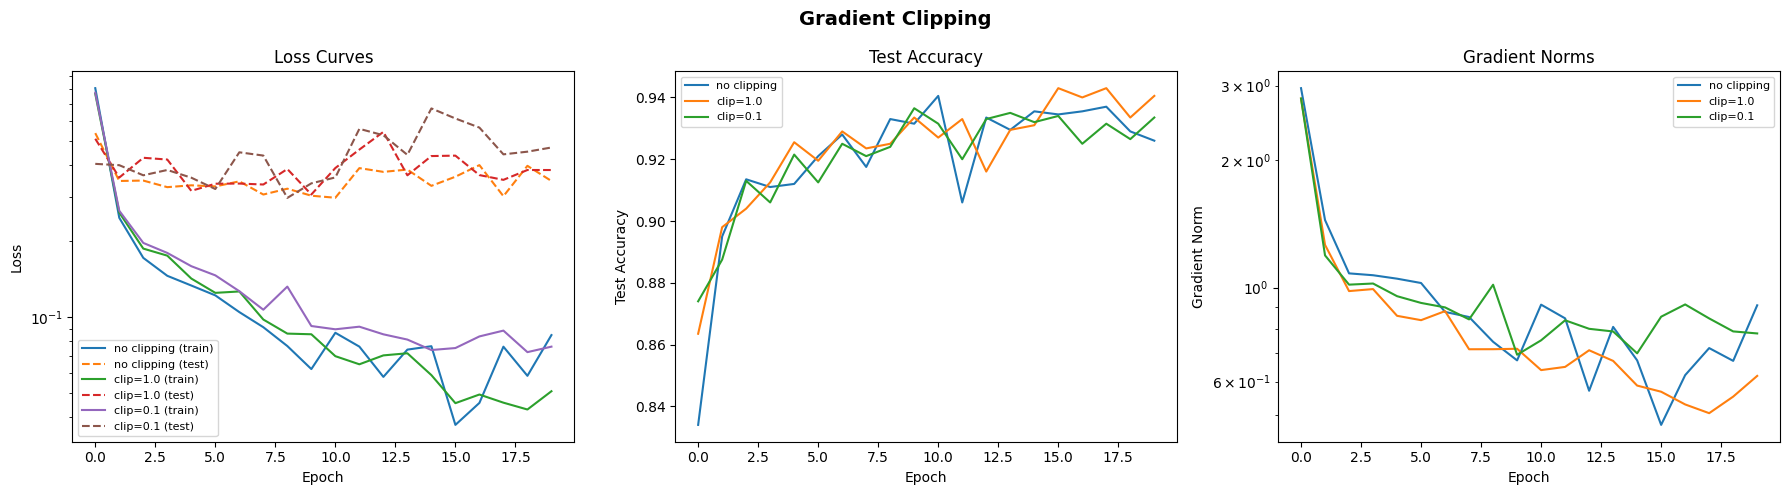
\includegraphics[width=\textwidth]{figures/gradient_clipping.png}
\end{center}

\vspace{2pt}
\small
Without clipping, gradient norms are volatile (right panel) and training is unstable.
\good{clip=1.0} tames the worst spikes while preserving learning speed.
\bad{clip=0.1} is too aggressive --- gradients are over-dampened and accuracy lags behind.

\end{frame}

% -------------------------------------------------------------------
\subsection{Gradient Accumulation}
% -------------------------------------------------------------------
\begin{frame}[fragile]{8.\ \ Gradient Accumulation}

\textbf{Problem:} you want effective batch size 256 but your GPU fits 64.

\vspace{4pt}
\textbf{Solution:} accumulate gradients over $k$ micro-batches before updating.

\begin{lstlisting}[style=python]
optimizer.zero_grad()
for i in range(accumulation_steps):          # e.g. 4
    loss = model(micro_batch[i]) / accumulation_steps
    loss.backward()                           # grads accumulate in .grad
optimizer.step()                              # one update
\end{lstlisting}

\[
  B_{\text{eff}} = B_{\text{micro}} \times k_{\text{accum}} \times n_{\text{GPUs}}
\]

\vspace{2pt}
\notebookcallout{10}{%
  Shows \texttt{bs=256} (actual) $\approx$ \texttt{bs=64 $\times$ 4 accum} (simulated) $\neq$ \texttt{bs=64} (no accum).%
}

\end{frame}

% -------------------------------------------------------------------
\begin{frame}{8.\ \ Gradient Accumulation --- Lab Results}

\begin{center}
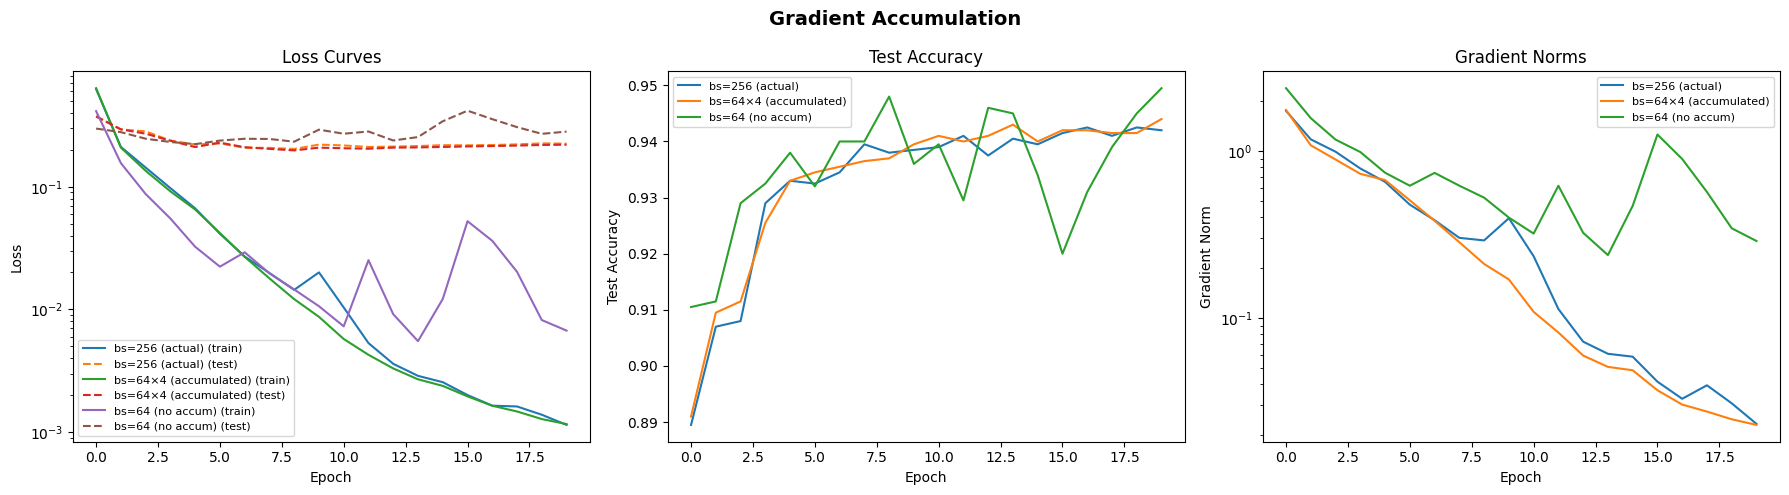
\includegraphics[width=\textwidth]{figures/gradient_accumulation.png}
\end{center}

\vspace{2pt}
\small
The \good{accumulated} run (orange, bs=64$\times$4) closely tracks the \good{actual bs=256} run (blue) in both loss and accuracy.
Plain bs=64 without accumulation (green) follows a different trajectory --- more parameter updates per epoch with noisier gradients.

\end{frame}

% -------------------------------------------------------------------
\subsection{Monitoring}
% -------------------------------------------------------------------
\begin{frame}{9.\ \ Monitoring: You Can't Optimize What You Can't See}

\begin{columns}[T]
\column{0.52\textwidth}
\textbf{What to track (wandb, TensorBoard)}

\begin{table}\scriptsize
\begin{tabular}{@{}ll@{}}
\toprule
\textbf{Metric} & \textbf{Signal} \\
\midrule
Train loss        & Is optimization working? \\
Val loss          & Is the model generalizing? \\
Train--val gap    & Overfitting? \\
Gradient norms    & Vanishing / exploding? \\
Learning rate     & Schedule behaving correctly? \\
GPU utilization   & Pipeline efficient? \\
\bottomrule
\end{tabular}
\end{table}

\column{0.44\textwidth}
\textbf{Red flags}

\vspace{4pt}
\bad{Loss flat} --- LR too low? Bug? \\[3pt]
\bad{Loss NaN} --- exploding grads \\[3pt]
\bad{Train $\downarrow$, val $\uparrow$} --- overfit \\[3pt]
\bad{Grad norm 0} --- vanishing \\[3pt]
\bad{Grad norm $\to\infty$} --- exploding

\end{columns}

\vspace{4pt}
\notebookcallout{11}{%
  Toggle \texttt{USE\_WANDB = True}; logs train/val loss, accuracy, gradient norms, and LR to a live dashboard.%
}

\end{frame}

% -------------------------------------------------------------------
\subsection{Regularization}
% -------------------------------------------------------------------
\begin{frame}{10.\ \ Regularization (Brief)}

Especially important for \keyword{small health datasets}:

\vspace{6pt}
\begin{description}[leftmargin=2.5cm]
  \item[Weight decay] L2 penalty on parameters. Built into AdamW.
  \item[Dropout] Randomly zero neurons during training. Forces redundancy.
  \item[Early stopping] Halt when val loss plateaus. Simple and effective.
  \item[Data augmentation] Synthetic variety (rotations, crops, masking). Especially for images.
\end{description}

\onslide<2->{
\vspace{4pt}
\begin{exampleblock}{Rule of thumb}
\good{Always} use weight decay (AdamW default). \\
\good{Overfitting?} Add dropout (0.1--0.5) and/or early stopping. \\
\good{Images?} Data augmentation is almost always worth it.
\end{exampleblock}
}

\end{frame}

% ===================================================================
\section{Putting It All Together}
% ===================================================================

% -------------------------------------------------------------------
\begin{frame}{A Training Recipe}

\begin{columns}[T]
\column{0.48\textwidth}
\begin{enumerate}
  \item Choose architecture (match modality)
  \item Initialize properly (Kaiming / Xavier)
  \item Add normalization + residual connections
  \item Start with \textbf{AdamW}, $\eta=10^{-3}$
  \item LR warmup (5--10\% of training)
\end{enumerate}

\column{0.48\textwidth}
\begin{enumerate}\setcounter{enumi}{5}
  \item Cosine or linear LR decay
  \item Gradient clipping (max norm 1.0)
  \item Gradient accumulation if memory-limited
  \item \textbf{Monitor everything} with wandb
  \item Evaluate on held-out data; early stop
\end{enumerate}
\end{columns}

\end{frame}

% -------------------------------------------------------------------
\begin{frame}{Summary}

\begin{itemize}
  \item<1-> Neural networks = \textbf{compositions of simple differentiable ops} --- the simplest function class satisfying universality + parametric + autodiff.
  \item<2-> Core unit: $\sigma(\bW\bx + \bb)$; depth $\times$ width $=$ expressiveness.
  \item<3-> \textbf{Architecture encodes inductive bias}: conv $\to$ locality; attention $\to$ learned interactions; MLP $\to$ no structural prior.
  \item<4-> Practical optimization requires \textbf{init + normalization + residuals + LR schedule + monitoring}.
  \item<5-> As the lab results show: each technique has a visible, measurable impact on training dynamics.
\end{itemize}

\onslide<6->{
\vspace{8pt}
\begin{center}
\Large\textcolor{AccentOrange}{\ding{118}}\quad
{\large\textbf{Notebook:} \texttt{nn\_fundamentals\_lab.ipynb} --- reproduce and extend every experiment}
\end{center}
}

\end{frame}

% ===================================================================
\appendix
% ===================================================================
{
  \setbeamertemplate{background canvas}[default]
  \setbeamercolor{background canvas}{bg=black}
  \begin{frame}[plain]
  \end{frame}
} 
% -------------------------------------------------------------------
\begin{frame}{What the Network Learns: First-Layer Weights}

\begin{center}
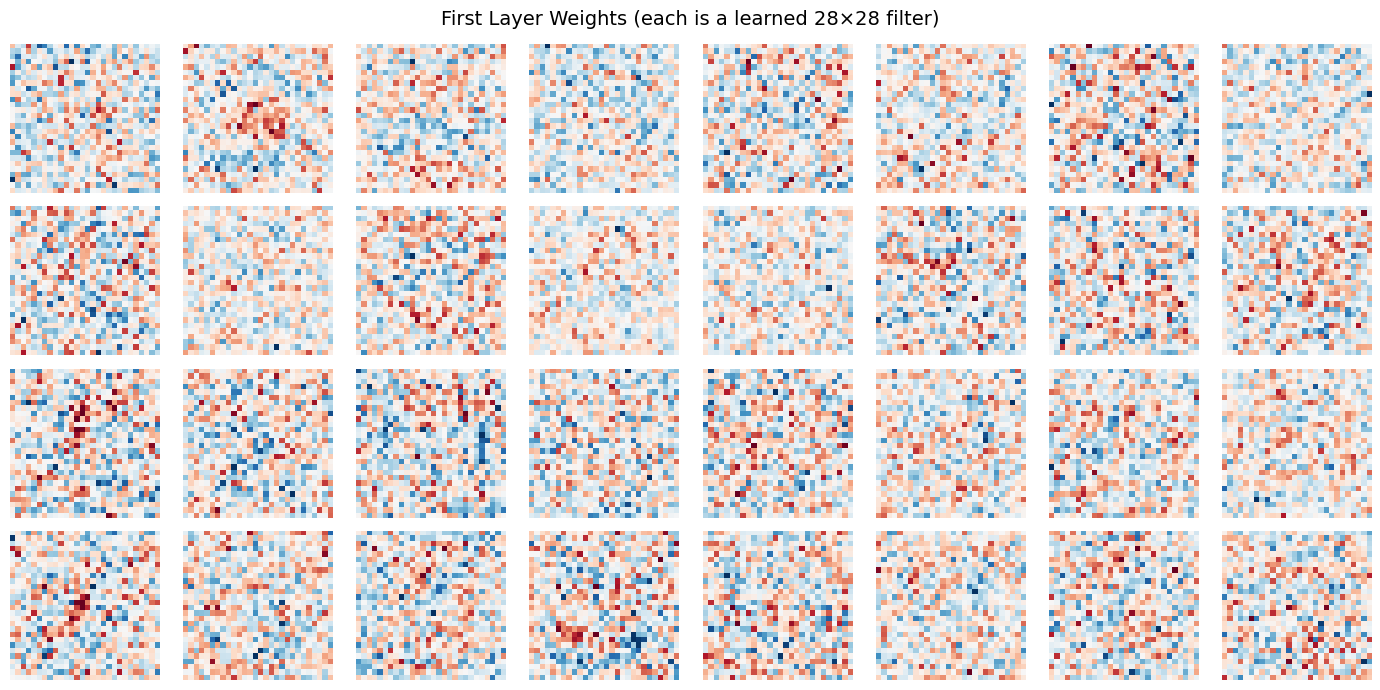
\includegraphics[width=0.78\textwidth]{figures/first_layer_weights.png}
\end{center}

\vspace{-2pt}
\small
Each $28\!\times\!28$ tile is one row of $\bW_1$ reshaped to image space --- the pattern that neuron responds to.
Some show stroke-like or edge features; others are harder to interpret.
Unlike CNN filters (local patches), MLP weights span the \keyword{entire image} --- no locality prior.

\end{frame}
% -------------------------------------------------------------------
\begin{frame}{What the Network Learns: Activations \& Predictions}

\begin{columns}[T]
\column{0.55\textwidth}
\textbf{Per-layer activations for a `7':}

\vspace{4pt}
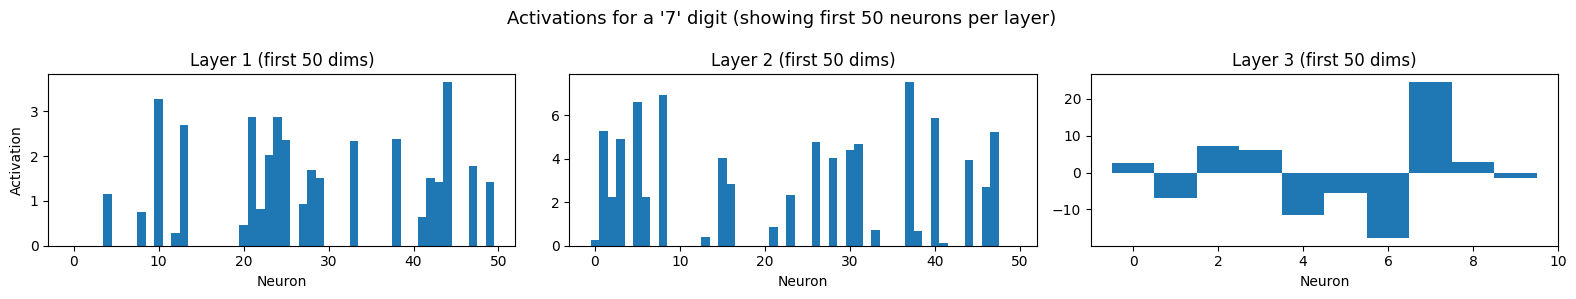
\includegraphics[width=\textwidth]{figures/activations_and_softmax.png}

\vspace{4pt}
\scriptsize
Layers 1 and 2 (after ReLU): sparse, non-negative. \\
Layer 3 (logits): 10 raw values, one per class --- both positive and negative.

\column{0.40\textwidth}
\textbf{Final softmax output:}

\vspace{4pt}
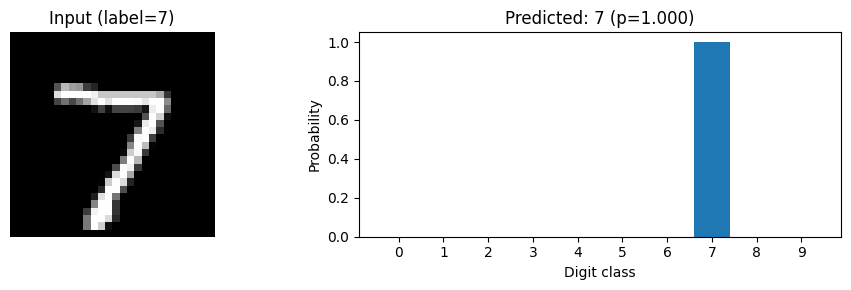
\includegraphics[width=\textwidth]{figures/activations_and_softmax_2.png}

\vspace{6pt}
\small
The network is \good{confident}: $p(\text{`7'}) \approx 1.0$.

\vspace{4pt}
This is the full pipeline: \\
pixels $\to$ features $\to$ logits $\to$ softmax $\to$ prediction.
\end{columns}

\end{frame}


\begin{frame}{Batch Size \& Learning Rate: The Full Picture}

The linear scaling rule (slide 6) is a \keyword{special case} of a deeper principle.

\vspace{4pt}
\begin{block}{The noise scale (Smith \& Le, 2017; Smith et al., 2018)}
SGD dynamics are governed by a \emph{noise scale}:
\[
  g \;=\; \frac{\varepsilon N}{B}
  \qquad\text{(vanilla SGD)},
  \qquad
  g \;=\; \frac{\varepsilon N}{B(1-m)}
  \qquad\text{(SGD + momentum)}
\]
where $\varepsilon$ is the learning rate, $N$ the dataset size, $B$ the batch size, and $m$ the momentum coefficient.
\end{block}

\vspace{4pt}
\textbf{Key insight:} Goyal's rule ($\varepsilon \propto B$) simply holds $g$ constant. But Smith et al.\ showed that \emph{decaying} the LR is equivalent to \emph{increasing} the batch size --- both reduce $g$.

\vspace{4pt}
\begin{alertblock}{Implication}
LR schedules are really \textbf{noise annealing} schedules. You can convert any LR decay into an equivalent batch-size increase --- same learning curves, fewer parameter updates.
\end{alertblock}

\vspace{2pt}
{\scriptsize Smith et al., ``Don't Decay the Learning Rate, Increase the Batch Size'' (ICLR 2018).}

\end{frame}

% -------------------------------------------------------------------
\begin{frame}{The Linear Scaling Rule Breaks Down for Adam}

The Goyal et al.\ linear rule ($\varepsilon \propto B$) was derived for \textbf{SGD}. Modern transformer training uses \textbf{AdamW}, where the dynamics are fundamentally different.

\vspace{6pt}
\begin{table}\centering\small
\begin{tabular}{@{}lll@{}}
\toprule
\textbf{Optimizer} & \textbf{Scaling rule} & \textbf{Source} \\
\midrule
SGD / SGD+momentum & $\varepsilon \propto B$ (linear) & Goyal et al., 2017 \\
Adam / AdamW       & $\varepsilon \propto \sqrt{B}$ (square root) & Malladi et al., 2022 \\
\bottomrule
\end{tabular}
\end{table}

\vspace{4pt}
\textbf{Why?} Adam normalizes updates by the second moment of gradients. Increasing $B$ reduces gradient variance, but Adam's denominator partially \emph{compensates} for this automatically --- so you need a smaller LR adjustment than with SGD.

\vspace{6pt}
\onslide<2->{
\begin{alertblock}{The ``surge'' phenomenon (Li et al., NeurIPS 2024)}
For Adam, the optimal LR is \bad{non-monotonic} in $B$: it first rises, then \emph{falls}, then converges to a constant. At very large $B$, Adam's update $\approx \text{sign}(\nabla\mathcal{L})$, which \textbf{saturates} --- adding more samples per step doesn't help.
\end{alertblock}
}

\end{frame}

% -------------------------------------------------------------------
\begin{frame}{Critical Batch Size: When Bigger Stops Helping}

\begin{block}{Critical Batch Size (McCandlish et al., 2018)}
There exists a \keyword{critical batch size} $B^*$ such that:
\begin{itemize}
  \item $B < B^*$: doubling $B$ roughly halves training steps (linear speedup).
  \item $B > B^*$: diminishing returns --- you pay more compute for marginal gains.
\end{itemize}
\end{block}

\vspace{4pt}
\textbf{What determines $B^*$?}
\begin{itemize}
  \item $B^*$ \good{grows during training} --- near zero at init, increases rapidly, then plateaus (Merrill et al., 2025). This naturally motivates \keyword{batch size warmup}.
  \item $B^*$ scales with \textbf{dataset size} more than model size (Zhang et al., 2024).
  \item For LLMs, $B^*$ can be very large ($10^4$--$10^6$ tokens), but McCandlish's gradient noise scale proxy is unreliable under Adam (Merrill et al., 2025).
\end{itemize}

\vspace{4pt}
\onslide<2->{
\begin{exampleblock}{Practical upshot}
Don't blindly maximize $B$. Use the largest batch size \textbf{below $B^*$} for your problem, scale LR accordingly, and consider ramping $B$ up during training.
\end{exampleblock}
}

\end{frame}

% -------------------------------------------------------------------
\begin{frame}{Putting It Together: Batch Size Strategy for Transformers}

\begin{columns}[T]
\column{0.50\textwidth}
\textbf{What the main slides teach} (correct!):
\begin{itemize}
  \item If you change $B$, rescale $\varepsilon$
  \item Grad accumulation $=$ larger effective $B$
  \item Warmup + cosine is a good default
\end{itemize}

\vspace{6pt}
\textbf{The fuller picture:}
\begin{itemize}
  \item LR decay $\equiv$ noise annealing $\equiv$ batch size increase (Smith et al., 2018)
  \item Use $\varepsilon \propto \sqrt{B}$ for AdamW, not linear
  \item There is a critical $B^*$ --- past it, you waste compute
  \item $B^*$ grows during training $\Rightarrow$ batch size warmup
\end{itemize}

\column{0.46\textwidth}
\textbf{Modern LLM recipe:}
\begin{enumerate}
  \item Start with small $B$ (high noise $=$ exploration)
  \item Ramp $B$ up over early training
  \item Cap at $B^*$ or hardware limit
  \item Use warmup + cosine LR decay on top
  \item This is \emph{two} annealing knobs, not one
\end{enumerate}

\vspace{6pt}
\begin{exampleblock}{Health AI context}
For small clinical datasets, $B^*$ is often small. \good{Linear scaling is fine as a starting heuristic.} For foundation model pre-training on EHR, the transformer-era nuances matter more.
\end{exampleblock}
\end{columns}

\end{frame}

% -------------------------------------------------------------------
\begin{frame}{Further Reading: Batch Size \& LR Scaling}

\begin{description}[leftmargin=0.4cm]
  \item[Noise scale] Smith \& Le, 2017 --- ``A Bayesian Perspective on Generalization and SGD''
  \item[Don't decay LR] Smith et al., 2018 --- ``Don't Decay the Learning Rate, Increase the Batch Size'' (ICLR 2018)
  \item[Critical BS] McCandlish et al., 2018 --- ``An Empirical Model of Large-Batch Training''
  \item[Adam scaling] Malladi et al., 2022 --- ``On the SDEs and Scaling Rules for Adaptive Gradient Algorithms'' (NeurIPS 2022)
  \item[Surge phenom.] Li et al., 2024 --- ``Surge Phenomenon in Optimal Learning Rate and Batch Size Scaling'' (NeurIPS 2024)
  \item[CBS revisited] Merrill et al., 2025 --- ``Critical Batch Size Revisited'' (NeurIPS 2025)
  \item[CBS \& data size] Zhang et al., 2024 --- ``How Does Critical Batch Size Scale in Pre-training?''
\end{description}

\end{frame}



% -------------------------------------------------------------------
% APPENDIX: Batch Size, LR, and Noise Scale --- The Full Picture
% -------------------------------------------------------------------

\begin{frame}{Batch Size \& Learning Rate: The Full Picture}

The linear scaling rule (slide 6) is a \keyword{special case} of a deeper principle.

\vspace{4pt}
\begin{block}{The noise scale (Smith \& Le, 2017; Smith et al., 2018)}
SGD dynamics are governed by a \emph{noise scale}:
\[
  g \;=\; \frac{\varepsilon N}{B}
  \qquad\text{(vanilla SGD)},
  \qquad
  g \;=\; \frac{\varepsilon N}{B(1-m)}
  \qquad\text{(SGD + momentum)}
\]
where $\varepsilon$ is the learning rate, $N$ the dataset size, $B$ the batch size, and $m$ the momentum coefficient.
\end{block}

\vspace{4pt}
\textbf{Key insight:} Goyal's rule ($\varepsilon \propto B$) simply holds $g$ constant. But Smith et al.\ showed that \emph{decaying} the LR is equivalent to \emph{increasing} the batch size --- both reduce $g$.

\vspace{4pt}
\begin{alertblock}{Implication}
LR schedules are really \textbf{noise annealing} schedules. You can convert any LR decay into an equivalent batch-size increase --- same learning curves, fewer parameter updates.
\end{alertblock}

\vspace{2pt}
{\scriptsize Smith et al., ``Don't Decay the Learning Rate, Increase the Batch Size'' (ICLR 2018).}

\end{frame}

% -------------------------------------------------------------------
\begin{frame}{The Linear Scaling Rule Breaks Down for Adam}

The Goyal et al.\ linear rule ($\varepsilon \propto B$) was derived for \textbf{SGD}. Modern transformer training uses \textbf{AdamW}, where the dynamics are fundamentally different.

\vspace{6pt}
\begin{table}\centering\small
\begin{tabular}{@{}lll@{}}
\toprule
\textbf{Optimizer} & \textbf{Scaling rule} & \textbf{Source} \\
\midrule
SGD / SGD+momentum & $\varepsilon \propto B$ (linear) & Goyal et al., 2017 \\
Adam / AdamW       & $\varepsilon \propto \sqrt{B}$ (square root) & Malladi et al., 2022 \\
\bottomrule
\end{tabular}
\end{table}

\vspace{4pt}
\textbf{Why?} Adam normalizes updates by the second moment of gradients. Increasing $B$ reduces gradient variance, but Adam's denominator partially \emph{compensates} for this automatically --- so you need a smaller LR adjustment than with SGD.

\vspace{6pt}
\onslide<2->{
\begin{alertblock}{The ``surge'' phenomenon (Li et al., NeurIPS 2024)}
For Adam, the optimal LR is \bad{non-monotonic} in $B$: it first rises, then \emph{falls}, then converges to a constant. At very large $B$, Adam's update $\approx \text{sign}(\nabla\mathcal{L})$, which \textbf{saturates} --- adding more samples per step doesn't help.
\end{alertblock}
}

\end{frame}

% -------------------------------------------------------------------
\begin{frame}{Critical Batch Size: When Bigger Stops Helping}

\begin{block}{Critical Batch Size (McCandlish et al., 2018)}
There exists a \keyword{critical batch size} $B^*$ such that:
\begin{itemize}
  \item $B < B^*$: doubling $B$ roughly halves training steps (linear speedup).
  \item $B > B^*$: diminishing returns --- you pay more compute for marginal gains.
\end{itemize}
\end{block}

\vspace{4pt}
\textbf{What determines $B^*$?}
\begin{itemize}
  \item $B^*$ \good{grows during training} --- near zero at init, increases rapidly, then plateaus (Merrill et al., 2025). This naturally motivates \keyword{batch size warmup}.
  \item $B^*$ scales with \textbf{dataset size} more than model size (Zhang et al., 2024).
  \item For LLMs, $B^*$ can be very large ($10^4$--$10^6$ tokens), but McCandlish's gradient noise scale proxy is unreliable under Adam (Merrill et al., 2025).
\end{itemize}

\vspace{4pt}
\onslide<2->{
\begin{exampleblock}{Practical upshot}
Don't blindly maximize $B$. Use the largest batch size \textbf{below $B^*$} for your problem, scale LR accordingly, and consider ramping $B$ up during training.
\end{exampleblock}
}

\end{frame}

% -------------------------------------------------------------------
\begin{frame}{Putting It Together: Batch Size Strategy for Transformers}

\begin{columns}[T]
\column{0.50\textwidth}
\textbf{What the main slides teach} (correct!):
\begin{itemize}
  \item If you change $B$, rescale $\varepsilon$
  \item Grad accumulation $=$ larger effective $B$
  \item Warmup + cosine is a good default
\end{itemize}

\vspace{6pt}
\textbf{The fuller picture:}
\begin{itemize}
  \item LR decay $\equiv$ noise annealing $\equiv$ batch size increase (Smith et al., 2018)
  \item Use $\varepsilon \propto \sqrt{B}$ for AdamW, not linear
  \item There is a critical $B^*$ --- past it, you waste compute
  \item $B^*$ grows during training $\Rightarrow$ batch size warmup
\end{itemize}

\column{0.46\textwidth}
\textbf{Modern LLM recipe:}
\begin{enumerate}
  \item Start with small $B$ (high noise $=$ exploration)
  \item Ramp $B$ up over early training
  \item Cap at $B^*$ or hardware limit
  \item Use warmup + cosine LR decay on top
  \item This is \emph{two} annealing knobs, not one
\end{enumerate}

\vspace{6pt}
\begin{exampleblock}{Health AI context}
For small clinical datasets, $B^*$ is often small. \good{Linear scaling is fine as a starting heuristic.} For foundation model pre-training on EHR, the transformer-era nuances matter more.
\end{exampleblock}
\end{columns}

\end{frame}

% -------------------------------------------------------------------
\begin{frame}{Further Reading: Batch Size \& LR Scaling}

\begin{description}[leftmargin=0.4cm]
  \item[Noise scale] Smith \& Le, 2017 --- ``A Bayesian Perspective on Generalization and SGD''
  \item[Don't decay LR] Smith et al., 2018 --- ``Don't Decay the Learning Rate, Increase the Batch Size'' (ICLR 2018)
  \item[Critical BS] McCandlish et al., 2018 --- ``An Empirical Model of Large-Batch Training''
  \item[Adam scaling] Malladi et al., 2022 --- ``On the SDEs and Scaling Rules for Adaptive Gradient Algorithms'' (NeurIPS 2022)
  \item[Surge phenom.] Li et al., 2024 --- ``Surge Phenomenon in Optimal Learning Rate and Batch Size Scaling'' (NeurIPS 2024)
  \item[CBS revisited] Merrill et al., 2025 --- ``Critical Batch Size Revisited'' (NeurIPS 2025)
  \item[CBS \& data size] Zhang et al., 2024 --- ``How Does Critical Batch Size Scale in Pre-training?''
\end{description}

\end{frame}
\end{document}